\documentclass[12pt]{article}

\usepackage{amsmath}

\usepackage[utf8]{inputenc}
\usepackage[T1, T2A]{fontenc}
\usepackage{fullpage}
\usepackage{multicol, multirow}
\usepackage{tabularx}
\usepackage{ulem}
\usepackage{listings}
\usepackage[english, russian]{babel}
\usepackage{tikz}
\usepackage{pgfplots}
\usepackage{indentfirst}
\usepackage{noindentafter}
\usepackage{nonfloat}
\usepackage{ulem}
\usepackage{fancyhdr}
% \usepackage{courier}
% \usepackage{FiraMono}
\usepackage{color}
\usepackage{subcaption}
\usepackage{titlesec}


\parindent=1cm

\linespread{1}
\pgfplotsset{compat=1.16}
\newcommand{\se}[1]{\section*{\bf #1}}

\newcommand{\listsource}[2]{
	\subsection*{\textbf{#2}}
	{\footnotesize
		\lstinputlisting[language=c++]{#1/#2}
	}
}

\lstdefinestyle{empty}{language=c++,
	basicstyle=\scriptsize,
	showspaces=false,
	showstringspaces=false,
	showtabs=false, вариантов
	tabsize=4,
	breaklines=true,
	escapechar=@,
	numbers=none,
	frame=none,
	escapeinside={\%*}{*)},
	breakatwhitespace=false % переносить строки только если есть пробел
}

\lstdefinestyle{customc}{
	belowcaptionskip=1\baselineskip,
	breaklines=true,
	frame=L,
	xleftmargin=\parindent,
	language=c++,
	numbers=left,
	showstringspaces=false,
	basicstyle=\footnotesize\ttfamily,
	keywordstyle=\bfseries\color{green!40!black},
	commentstyle=\itshape\color{purple!40!black},
	identifierstyle=\color{blue},
	stringstyle=\color{orange},
}

\lstset{escapechar=@,style=customc}

\pgfplotsset{compat=1.17}

\titleformat{\section}
{\normalfont\Large\bfseries}{\thesection.}{0.3em}{}

\titleformat{\subsection}
{\normalfont\large\bfseries}{\thesubsection.}{0.3em}{}

% \titlespacing{\section}{0pt}{*2}{*2}
% \titlespacing{\subsection}{0pt}{*1}{*1}
% \titlespacing{\subsubsection}{0pt}{*0}{*0}
% \lstloadlanguages{Lisp}
% \lstset{extendedchars=false,
% 	escapechar= |,
% 	breaklines=true,
% 	breakatwhitespace=true,
% 	keepspaces = true,
% 	tabsize=2
% }

\newcommand{\makemytitlepage}[2]{
	\thispagestyle{empty}
	\begin{center}
		\bfseries

		{\Large Московский авиационный институт\\ (национальный исследовательский университет)

		}

		\vspace{48pt}

		{\large
			Институт №8 ``Информационные технологии и прикладная математика''
			Кафедра 806 ``Вычислительная математика и программирование''
		}

		\vspace{36pt}

		{Лабораторная работа №#1  \\
			По курсу ``Программирование графических процессоров''
		}
		\vspace{48pt}

		{#2}

	\end{center}

	\vspace{72pt}

	\begin{flushright}
		\begin{tabular}{rl}
			Выполнил:      & П.\, А. Милько      \\
			Группа:        & М8О-408Б-17         \\
			Преподаватели: & К.Г. Крашенинников, \\
			               & А.Ю. Морозов.       \\
		\end{tabular}
	\end{flushright}

	\vfill

	\begin{center}
		\bfseries
		Москва\\
		\the\year
	\end{center}
	\newpage
	\setcounter{page}{1}
}

\newcommand{\nvidia}[0]{
	\se{Программное и аппаратное обеспечение}
	
	TODO
}

\begin{document}
\makemytitlepage{3}{Классификация и кластеризация изображений на GPU.}

\se{Цель работы}

Научиться использовать GPU для классификации и
кластеризации изображений. Использование константной памяти.

\textbf{Вариант 5.} Метод k-средних.

\textbf{Входные данные.}
На первой строке задается путь к исходному изображению,
на второй, путь к конечному изображению. На следующей строке, число $nc$ -- кол-во
кластеров. Далее идут $nc$ строчек описывающих начальные центры кластеров. Каждая
i-ая строчка содержит пару чисел -- координаты пикселя который является центром.
$nc <= 32$.

\nvidia

\se{Метод решения}

Метод k-средних простой как палка.
Нужно всего лишь каждый пиксель сопоставить с ближайшим по цвету кластером.
Изначальные цвета кластеров задаются явно, либо выбираются из случайных пикселей изображения.

Вся прелесть алгоритма в том что в процессе работы центры классов могут изменяться в зависимости
от принадлежащих кластеру точек. Получается некоторый ``средний вес''.

Очевидно что алгоритм не отработает за одну итерацию, если центры могут перемещаться.

Но чтобы алгоритм всё таки мог завершиться нужно условие выхода:

\begin{enumerate}
	\item Правильное условие: на текущей итерации все пиксели принадлежат тем же классам, каким принадлежали
	      на предыдущей итерации.
	\item Простое условие: новые значения центров классов отличаются по норме не более чем на
	      $\varepsilon$ от предыдущих значений.
\end{enumerate}

Второе условие всё же более предпочтительно, т.к. классов будет явно меньше чем пикселей.

\se{Описание программы}

\subsubsection*{Созданные ядра:}

\begin{itemize}
	\item \lstinline|kernel| --- название красноречиво. Сопоставляет каждый пиксель
	      его ближайшему классу, точнее аккумулирует значения пикселей класса в небольшой кеш,
	      равный по размеру количеству классов.
	\item \lstinline|calc_centers| --- вычисление новых центров классов, которое основывается
	      на кеше, полученном от первого ядра. Тут же проверяется близость новых центров классов и старых.
\end{itemize}

\subsubsection*{Дополнительные условия:}

По условиям лабораторной следует использовать константную память.

Так как размер её ограничен (64КБ), то записать в неё изображение не получится.

А вот центры классов будут очень даже хорошо смотреться в константной памяти,
так как их немного и они все постоянно используются в первом ядре.

{
\listsource{../src}{main.cu}
}

\se{Результаты}

\begin{figure}[!tbh]
	\caption*{Малое изображение: 400x408}
	\begin{subfigure}{0.49\textwidth}
		\centering
		\caption*{Исходное изображение}
		
\includegraphics[scale=0.4]{../test/images/nigger.png}
	\end{subfigure}
	\begin{subfigure}{0.49\textwidth}
		\centering
		\caption*{Результат:}
		
\includegraphics[scale=0.4]{t3-res.png}
	\end{subfigure}
\end{figure}

Были выделены пиксели с отдельных лепестков и из центральной области.

\begin{figure}[!tbh]
	\caption*{Большое изображение: 6000x4000}
	\begin{subfigure}{0.49\textwidth}
		\centering
		\caption*{Исходное изображение}
		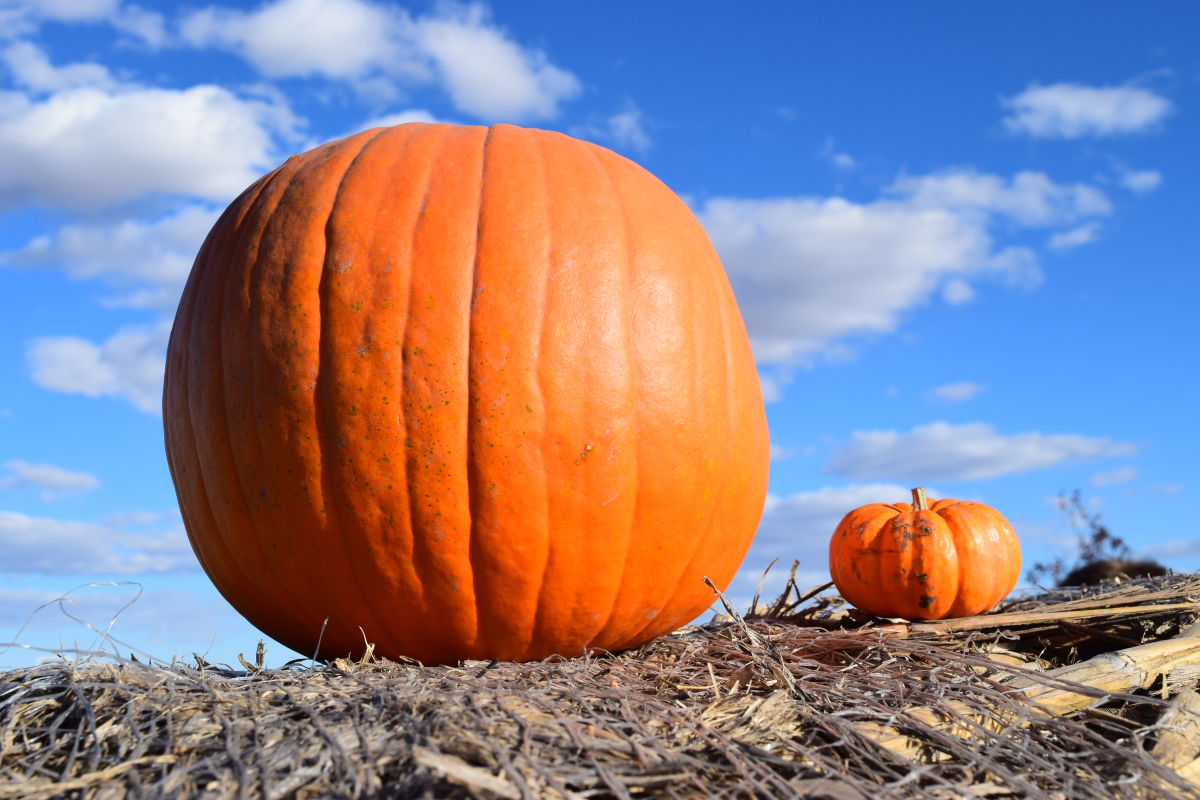
\includegraphics[scale=0.79]{pp.png}
	\end{subfigure}
	\begin{subfigure}{0.49\textwidth}
		\centering
		\caption*{Результат:}
		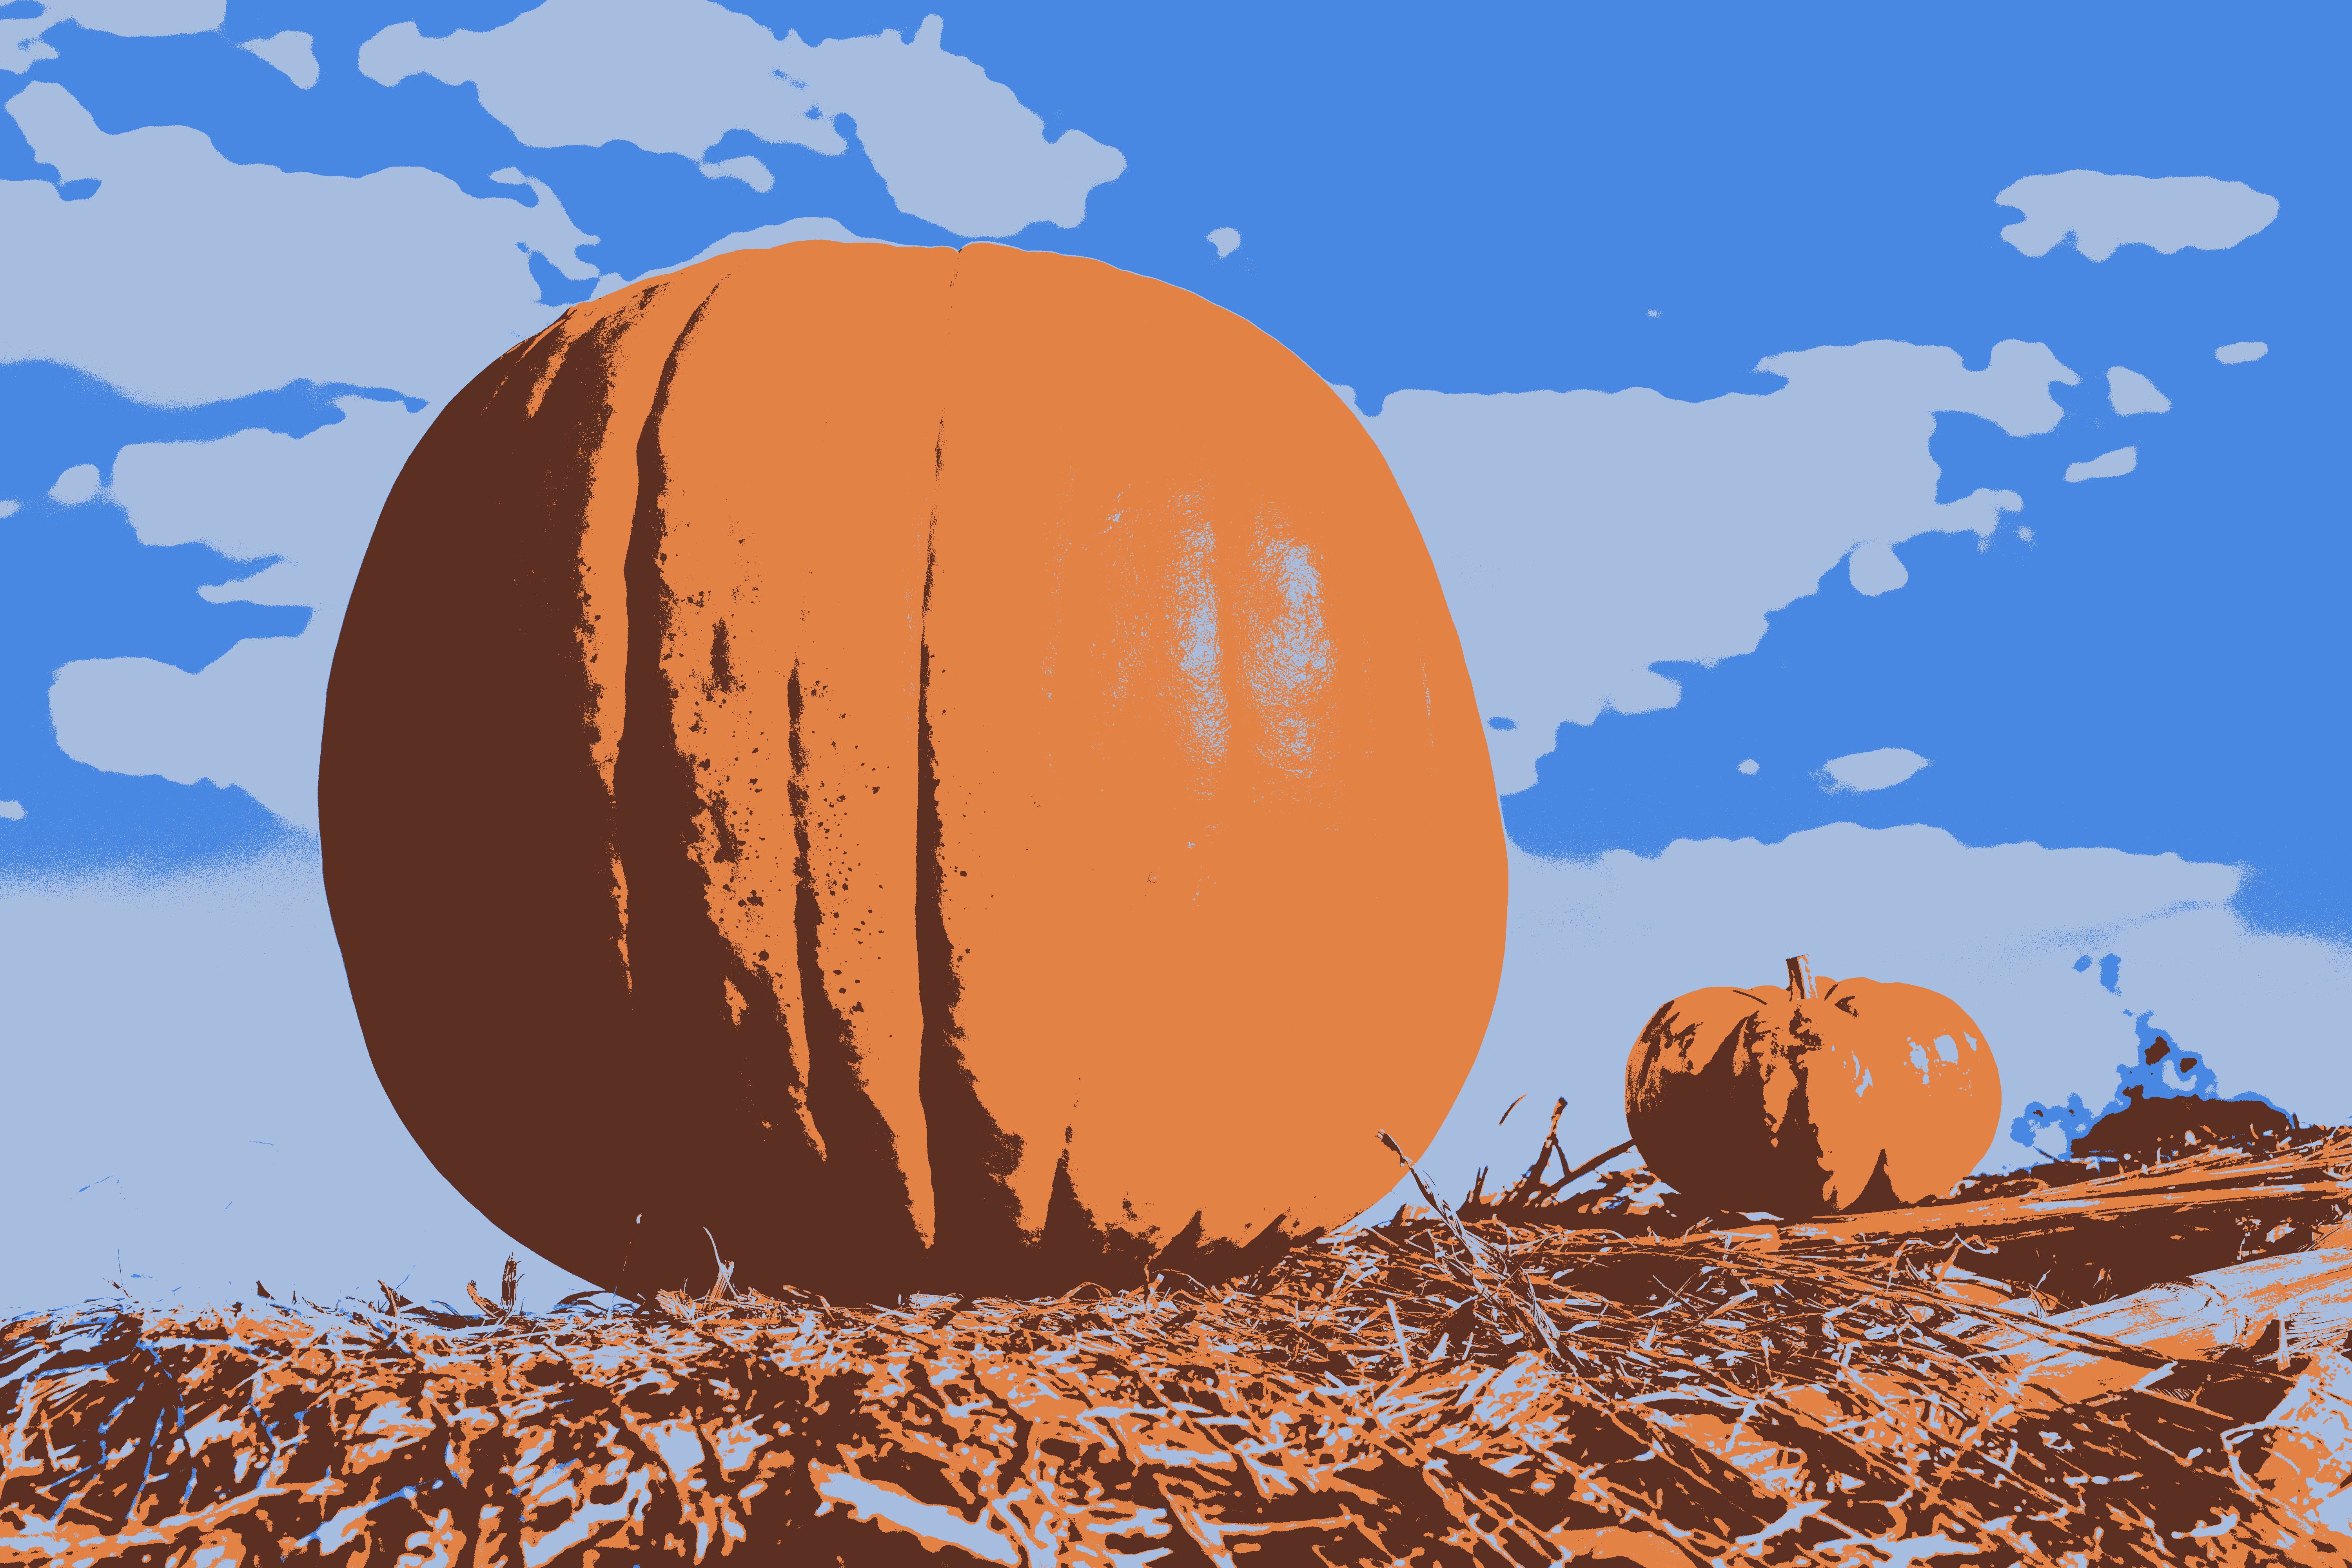
\includegraphics[scale=0.038]{pumpkin-result.png}
	\end{subfigure}
\end{figure}

Были выделены пиксели на облаке, чистом небе, тыкве и соломе.
Но так получилось что цвет соломы оказался несколько ближе к цвету тыквы.

\newpage

\textit{Время указано в миллисекундах}

Малое изображение:

\begin{center}
	cpu time = 6.437255
	\begin{table*}[!htb]
		\centering
		\begin{tabular}{|c|c|c|}
			\hline
			blocks & threads & time        \\
			\hline

			1      & 32      & 201.184063  \\
			16     & 16      & 290.349113  \\
			32     & 32      & 2561.765715 \\
			32     & 64      & 296.941000  \\
			64     & 64      & 146.438572  \\
			64     & 128     & 140.186692  \\
			128    & 1024    & 139.336220  \\
			1024   & 1024    & 142.516288  \\
			\hline
		\end{tabular}
	\end{table*}
\end{center}

Большое изображение:

\begin{center}
	cpu time = 4737.693401
	\begin{table*}[!htb]
		\centering
		\begin{tabular}{|c|c|c|}
			\hline
			blocks & threads & time         \\
			\hline

			1      & 32      & 84191.246064 \\
			16     & 16      & 7494.419552  \\
			32     & 32      & 3855.833430  \\
			32     & 64      & 4167.838969  \\
			64     & 64      & 5816.296628  \\
			64     & 128     & 3968.485597  \\
			128    & 1024    & 3962.384164  \\
			1024   & 1024    & 3965.347436  \\
			\hline
		\end{tabular}
	\end{table*}
\end{center}

\se{Выводы}

Тут разрыв с CPU не столь явный, скорее всего виноваты атомарные операции сложения,
потому что из за малого количества классов они будут обращаться к одной и той же памяти
последовательно.

Ну главное что оно работает.

В будущем постараюсь столь плохо не делать.

\end{document}